\chapter{Preliminary Work}\label{ch:Preliminary}

\section{Task 1: Graph KSVD}

Sparse representation is a technique used to learn a dictionary that lies in the original feature domain and calculate a sparse representation using a linear combination of a few dictionary elements (atoms)\cite{Elad2010}. %\cite{Elad2010, Zhang2015}.
The main advantages of using sparse representation are linearity and sparsity: the learned embedding consists of linear combinations of sub-tree structures; sparse representations allow using low-order classifcation models due to the low VC dimension\cite{Neylon2006}. Sparse representation was originally introduced in the signal and image processing domains, however recently it has been utilized in graph-related processes. Several methods have been proposed to represent graph signals on a fixed graph topology with sparse representations with theoretical guarantees\cite{Yankelevsky2019}. %\cite{Subbareddy2019, Thanou2013, Zhang2021, Yankelevsky2020}.
Recent work by Matsuo et al.\cite{Matsuo2019} develops a method to represent different network topologies with sparse representation. However, their work is still limited by requiring graphs to be undirected and requiring all topologies to have the same number of nodes.

To address the shortcomings in sparse vector-based graph representations, we introduce a framework to incorporate WL sub-tree kernel with sparse representation methods specifically aimed at machine learning classification tasks. Our framework allows sparse representation to be applied to graphs with different topologies and different numbers of nodes. In addition, the input graphs can be directed and can incorporate node features. An overview of the proposed WL+KSVD pipeline is shown in Fig.\ref{fig: GKSVD}. The proposed method has the flexibility to swap different dictionary learning and graph kernel methods in the framework. The method is tested against several similar graph embedding methods with benchmark datasets. Finally, the python implementation of the framework and the experiments are currently available on Github\footnote{\url{https://github.com/BMW-lab-MSU/WL-KSVD.git}}.

\begin{figure}[!tbh]
\centerline{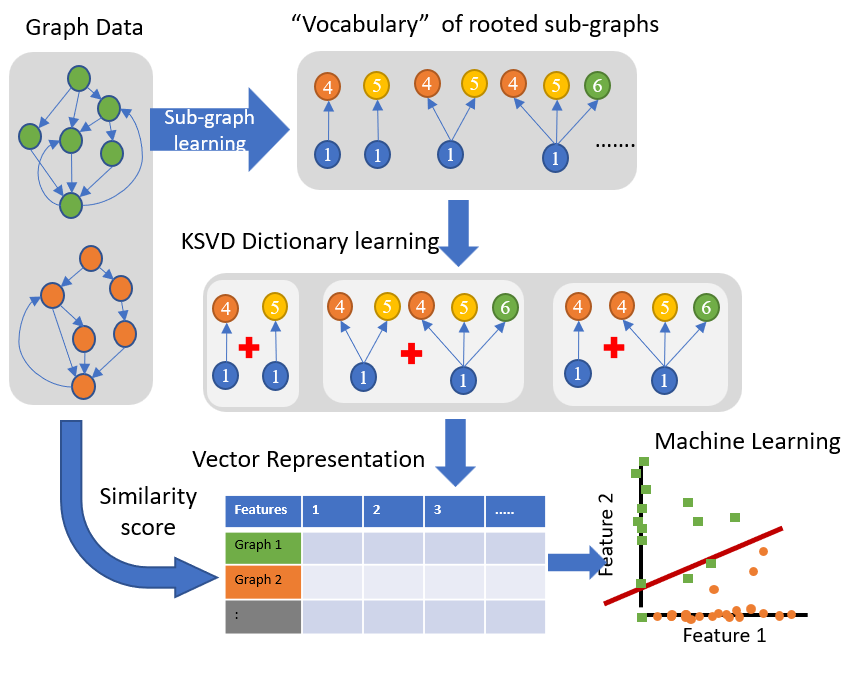
\includegraphics[width=0.9\columnwidth]{figures/Graph_embedding/GraphKSVD.png}}
\caption{Proposed WL+KSVD pipeline overview}\label{fig: GKSVD}
\end{figure}

\begin{figure}[!tbh]
\centerline{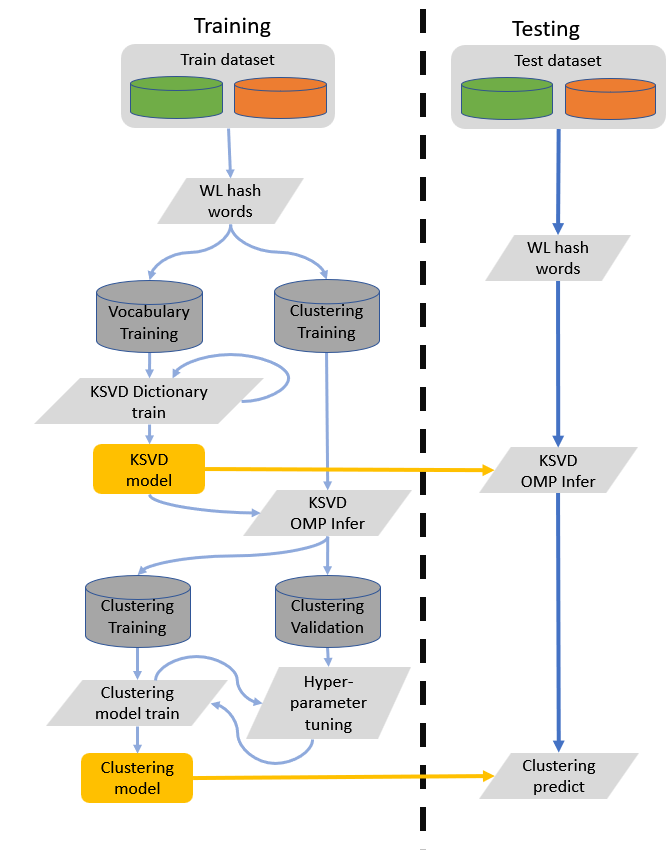
\includegraphics[width=0.7\columnwidth]{figures/Graph_embedding/Workflow.png}}
\caption{Evaluation Workflow}\label{fig: workflow}
\end{figure}

\subsection{Methodology}

An overview of the workflow of the proposed method is shown in Fig.\ref{fig: workflow}, where the training set is further divided in half into embedding training and classifier training to avoid over fitting.

\subsection{Graph Notation and Definition}
Let a graph be defined as $G = (V, E)$ which can be directed or undirected with unweighted edges, where node $v_i \in V$ and edge $e_{i,j} \in E$ connects $v_i$ and $v_j$. Let the dataset be a set of $M$ graphs with different topology and nodes $\mathbf{G} = [G_1, G_2, \dots, G_M]$. Following the Graph2Vec algorithm, ff node labels are not provided the nodes will be initialized with the degree of the node as its label. The degree of a node is a count of the number of edges the node receives and sends. We use the ``NetworkX'' python package as the graph data structure\footnote{\url{https://networkx.org/}}.

\subsection{Weisfeiler-Lehman sub-tree  kernel}

WL sub-tree relabelling process (described in\cite{shervashidze2011weisfeiler}\footnote{\url{https://github.com/benedekrozemberczki/karateclub/blob/master/karateclub/utils/treefeatures.py}}) is used to relabel the nodes with a unique hash value for the rooted sub-tree structure. Note that the sub-tree structure learned is deterministic, so the same sub-tree structure in different graphs will have the same hash value. For each $G_i \in \mathbf{G}$, rooted sub-trees $sg_{i,j}^h$ are learned for each $v_j \in \mathbf{V}_i$, where $i$ is the graph, $j$ is the node and $h$ is the WL rooted sub-tree depth. Now each graph is a set of hash words $G_i = [sg_{1,i}^h, sg_{2,i}^h, \dots, sg_{l,i}^h]$, where $l_i$ is the number of nodes in $G_i$.

\subsection{Vocabulary Creation}
Using the Doc2Vec implementation in Gensim python package\footnote{\url{https://radimrehurek.com/gensim/}} a raw vocabulary is created using the unique set of sub-tree hash words $sg$ across all the training graphs\cite{Le2014}. If the raw vocabulary is too large it can be trimmed according to a trim rule. In this work, we trim the vocabulary by selecting the $K$ highest frequency sub-tree hash words. Other possible trimming rules are the highest likelihood, highest prior, etc. 

Each graph $G_i$ is then represented as the occurrences $Y_i$ of the vocabulary elements, where $Y_i = [y_{i,1}, \dots , y_{i,K}]$ and $y_{i,j}$ is the number of occurrences of vocabulary word $j$ in graph $i$. Now the dataset can be represented as a collection of fixed-length vectors: $\mathbf{Y} = [Y_1, Y2, \dots , Y_M] \in \mathbb{R}^{K \times M}$.


\subsection{Sparse Representation}

Let $\mathbf{Y} = [Y_1, Y_2, \dots, Y_M] \in \mathbb{R}^{K \times M}$ be a set of $M$ input signals with fixed length $K$. Sparse representation attempts to represent the input signal as a linear combination of elements $d_i \in \mathbb{R}^{K}$ in a dictionary $\mathbf{D} = [d_1, d_2, \dots , d_N] \in \mathbb{R}^{K \times N}$ while limiting the number of atoms used to $T$ (sparsity). The sparse coefficient vector $\mathbf{\alpha} = [\alpha_1, \alpha_2, \dots \alpha_M] \in \mathbb{R}^{K \times M}$ will be the sparse representation with $|\alpha_i|_0 \leq T$, where $|.|_0$ operator counts the number of non-zero elements in the vector. The general form of the sparse representation can be formulated as:
\begin{align}
\label{eqn: SR}
    \argmin_{\mathbf{D}, \mathbf{\alpha}} || \mathbf{Y} - \mathbf{D\alpha}||_2^2 + ||\mathbf{\alpha}||_0.
\end{align}
This equation is NP-hard, but an approximate solution can be provided using an iterative algorithm named K-means Singular Value Decomposition (KSVD)\cite{Aharon2006}\footnote{\url{https://github.com/nel215/ksvd}}. First, a dictionary $\mathbf{D}$ is fixed and sparse vectors $\mathbf{\alpha}$ are optimized using Orthogonal Matching Pursuit (OMP)\cite{Pati1993}. Second, $\mathbf{\alpha}$ is fixed and the dictionary $\mathbf{D}$ is updated with a generalized K-means algorithm. After many iterations, each graph is represented as a fixed-length \emph{sparse} vector. In addition, using the trained dictionary, new graphs can be represented as sparse vectors.


\section{Task 2: Feature Ranking}

\subsection{Proposed Sparse Representation Based FR metrics}

Figure\ref{fig: D_metrics} shows the linear mapping of the dictionary elements and weighted dictionary elements to the original input space. Even though the metrics are simple projections of the dictionary elements into input space, Learning dictionary elements are complex. The dictionary elements are learned through the KSVD algorithm iteratively optimizing, considering all the training samples. Hence the learned dictionary elements capture the common patterns in the dataset. 


\begin{figure*}[!t]%
\centering
\subfloat[\emph{dictionary mapping}]{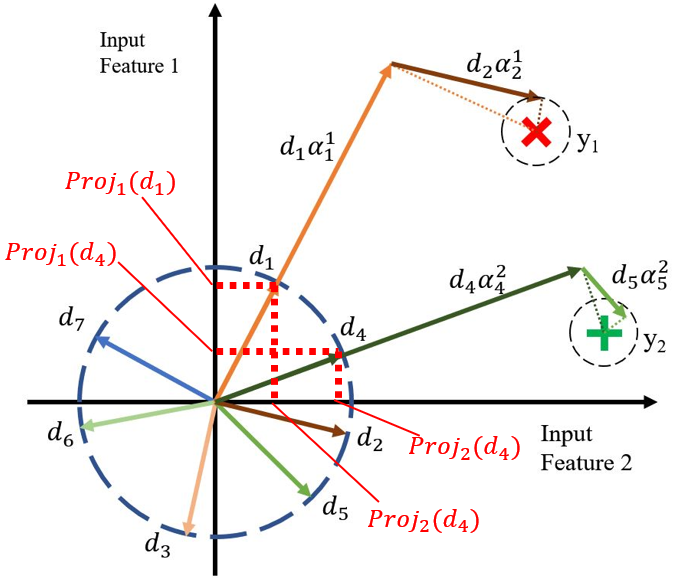
\includegraphics[width=0.4\columnwidth]{Figures/D_map.png}}\label{subfig: D_map}%
\qquad
\subfloat[\emph{dictionary utilization}]{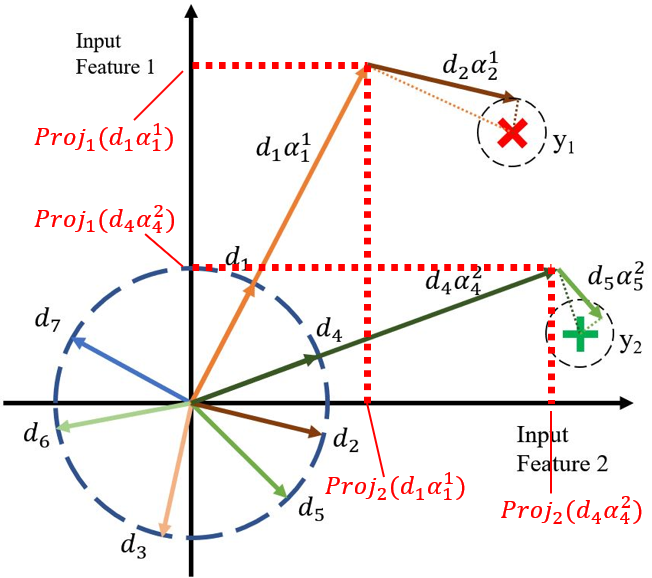
\includegraphics[width=0.4\columnwidth]{Figures/D_util.png}}\label{subfig: D_util}
\caption{Projection of dictionary elements and weights into input space. (a) \emph{dictionary mapping} only projects the dictionary atoms. (b) \emph{dictionary utilization} projects the weighted dictionary atoms according to the sparse representation.}%
\label{fig: D_metrics}%
\end{figure*}


\subsubsection{Dictionary mapping}

First \emph{Dictionary mapping}, $\mathbf{D}_\textrm{map} \in \mathbb{R}^{1 \times d}$, which calculates the sum of the squares of the projections of the dictionary atoms for each feature as given in (\ref{eq:dict_map}), where $\Proj_j$ is the projection operator into feature $F_j$. 

\begin{equation}
    \label{eq:dict_map}
    \mathbf{D}_\textrm{map}(j)= \sum_{i=1}^m {\Proj_j(d_i)}^2  = \sum_{i=1}^m {\mathbf{D}_{(j,i)}}^2 
\end{equation}

Figure\ref{fig: D_metrics}.a shows the projections used for \emph{dictionary mapping}.The Sum of squares of the projections is used to calculate the metric. More dictionary elements will be concentrated in subspaces where the data is highly distributed. We hypothesize features with high variance should have a higher \emph{dictionary mapping} score. This proposal will try to find mathematical and experimental validation for this claim.

\subsubsection{Dictionary utilization}
 The second metric is the \emph{Dictionary utilization}, $\mathbf{D}_\textrm{util} \in \mathbb{R}^{1 \times d}$, which calculated the utilization of the dictionary elements by the sparse coefficients. This acts as a weighted measure of the \emph{dictionary mapping}. Finally, the weighted dictionary atoms are projected back to their original features. The equation is given in (\ref{eq:dict_util}).

 
 \begin{equation}
    \label{eq:dict_util}
    \mathbf{D}_\textrm{util}(j)= \sum_{i=1}^m \Proj_j(d_i \cdot \sum_{k=1}^n |\alpha_{j,k}|)  
\end{equation}

Figure Figure\ref{fig: D_metrics}.b shows the projections used for \emph{dictionary utilization}. Since we are learning an over-complete dictionary and representing data sparsely, Not all the dictionary atoms are used all the time. Hence, understanding which dictionary atoms are used by the sample can give insight into common patterns and rare occurrences. If identify the dictionary atom usage b class, we can develop class-wise feature importance. The more the dictionary atom is used the higher the score for its relevant feature.


%%%%%%%%%%%%%%%%%%%%%%%%%%%%%%%%%%%%%%%%%%%%%%%%%%%%%%%%%%%%%%%
%%%%%%%%%%% Figures placed here for formatting %%%%%%%%%%%%%%%%
%%%%%%%%%%%%%%%%%%%%%%%%%%%%%%%%%%%%%%%%%%%%%%%%%%%%%%%%%%%%%%%
\begin{figure}[!t]%
    \centering
    \subfloat[][]{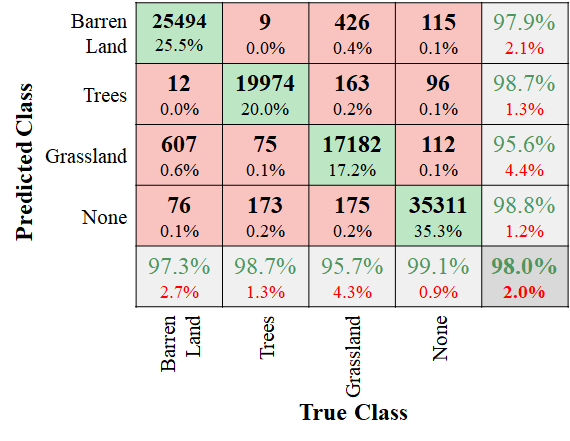
\includegraphics[width=0.3\columnwidth]{figures/SR/S4_FZN.png}}%
    \qquad
    \subfloat[][]{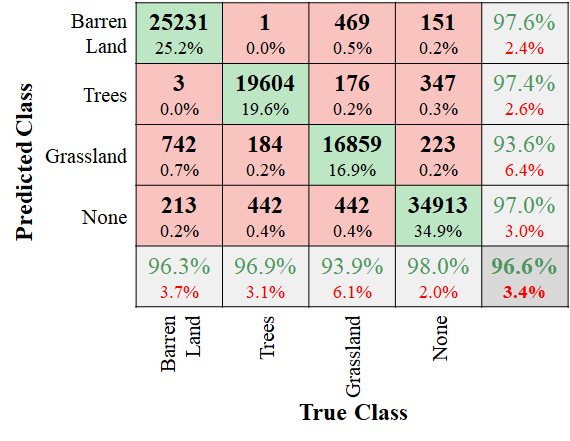
\includegraphics[width=0.3\columnwidth]{figures/SR/S4_LCK.png}}\\\label{fig: sat4_rslt}%
    
    %\ContinuedFloat
    
    \subfloat[][]{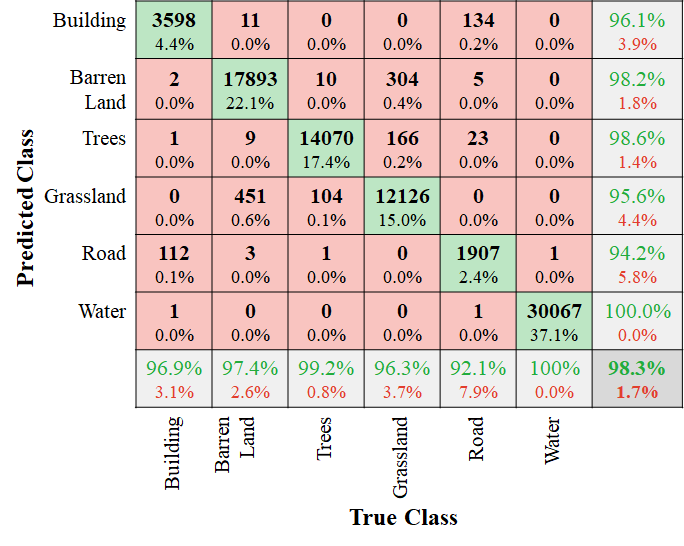
\includegraphics[width=0.4\columnwidth]{figures/SR/S6_FZN.png}}%
    \qquad
    \subfloat[][]{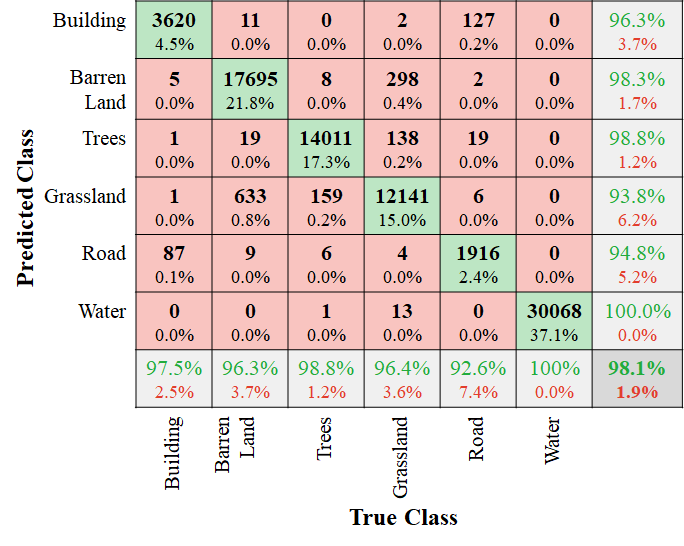
\includegraphics[width=0.4\columnwidth]{figures/SR/S6_LCK.png}}
    \caption[]{Confusion matrix for the Sat-4 (a,b) and Sat-6 (c,d) datasets with Frozen (a,c) and LC-KSVD (b,d) dictionary learning methods.}%
    \label{fig: sat6_rslt}%
    \end{figure}
    %%%%%%%%%%%%%%%%%%%%%%%%%%%%%%%%%%%%%%%%%%%%%%%%%%%%%%%%%%%%%%%
    %%%%%%%%%%%%%%%%%%%%%%%%%%%%%%%%%%%%%%%%%%%%%%%%%%%%%%%%%%%%%%%
    
    
    
    
    
    
    Let $\mathbf{F} = [F_1, F_2, \dots F_d]$ be a set of $d$ features $F$ which are collected or curated. The goal is to rank the feature set $\mathbf{F}$ by evaluating a mean-removed training set of $n$ samples: $\mathbf{\bar{X}} = [x_1, x_2, \dots, x_n] \in \mathbb{R}^{d \times n}$. The set of $k$ classes is defined as $\mathbf{C} = [C_1, C_2, \dots, C_k]$, where each of the $x$ samples is assigned to a class $C$. In sparse representation the input sample is represented as a linear combination of dictionary elements $D$ in a over-complete ($d \ll m$) dictionary $\mathbf{D} = [D_1, D_2, \dots, D_m] \in \mathbb{R}^{d \times m}$, where the number of dictionary elements used, $s$, is far less than the number of dictionary atoms: $s \ll m$. The set coefficients $\bm{\alpha} = [\alpha_1, \alpha_2, \dots, \alpha_n] \in \mathbb{R}^{m \times n}$ of the linear combination is called the sparse coefficients. Each coefficient vector contains $s$ nonzero entries; the remaining $m-s$ entries are exactly zero. The general objective function used for calculating the sparse representation is given by (\ref{eq:sparse}) with an $\ell_0$ constraint on sparsity.
    
    \begin{equation}
        \label{eq:sparse}
        \argmin_{\mathbf{D},\bm{\alpha}} ||\mathbf{\bar{X}}- \mathbf{D}\bm{\alpha}||_F + ||\bm{\alpha}||_0
    \end{equation}
    
    The KSVD algorithm is an efficient iterative method that solves the objective function by, first fixing the $\mathbf{D}$ and optimizing the $\bm{\alpha}$ using orthogonal matching pursuit (OMP)\cite{Pati1993}. Second, it fixes $\bm{\alpha}$ then optimize $\mathbf{D}$ with generalized K-means and singular value decomposition (SVD). Since the learned dictionary is over-complete, the spread of the dictionary atoms can give an insight into which features are more relevant for the representation. Hence, we will be defining simple metrics that will quantify the spread of the dictionary elements in each of the features. First \emph{Dictionary mapping}, $\mathbf{D}_\textrm{map} \in \mathbb{R}^{1 \times d}$, which calculates the sum of the squares of the projections of the dictionary atoms for each feature as given in (\ref{eq:dict_map}), where $\Proj_j$ is the projection operator into feature $F_j$. 
    
    % \begin{equation}
    %     \label{eq:dict_map}
    %     \mathbf{D}_\textrm{map}(j)= \sum_{i=1}^m {\Proj_j(D_i)}^2  = \sum_{i=1}^m \mathbf{D}_{(j,i)}^2 
    % \end{equation}
    
     The second metric is the \emph{Dictionary utilization}, $\mathbf{D}_\textrm{util} \in \mathbb{R}^{1 \times d}$, which calculated the utilization of the dictionary elements by the sparse coefficients. This acts as a weighted measure of the \emph{dictionary mapping}. Finally, the weighted dictionary atoms are projected back to original features. The equation is given in (\ref{eq:dict_util}).
     
    %  \begin{equation}
    %     \label{eq:dict_util}
    %     \mathbf{D}_\textrm{util}(j)= \sum_{i=1}^m \Proj_j(D_i \cdot \sum_{k=1}^n |\alpha_{j,k}|)  
    % \end{equation}
     
    The KSVD algorithm learns the dictionary in an unsupervised manner, hence we cannot get dictionary elements that are optimized for class discrimination. Therefore several other methods have been proposed to learn a more discriminative dictionary by learning in a supervised manner, giving us a strong association of dictionary atoms with each class. Here we will be exploring two such methods, LC-KSVD and Frozen KSVD\@. By doing so we can decompose the proposed metrics into classes, which gives more insight into feature behavior concerning class labels. In LC-KSVD the algorithm enforces two extra constraint terms related to dictionary association with each class and linear classifier performance. Hence, samples are forced to utilize a subset of the dictionary atoms for their representation leading to a more discriminatory dictionary. However, when imbalanced data is presented the LC-KSVD algorithm does not change the dictionary atom distribution. Therefore, Frozen KSVD is proposed to take class imbalances into consideration of dictionary learning. It first learns a dictionary only considering the largest class. Then next largest class is trained with added dictionary atoms while keeping the previously learned dictionary atoms fixed (frozen). This forces the algorithm to learn new dictionary atoms which are associated with only the new class. This is repeated for all the classes such that the added number of dictionary atoms and the sparsity of each class are reduced depending on the class size. 

    subsection{Dictionary Elements Analysis}

% \begin{figure*}[!t]%
% \centering
% \subfloat[][]{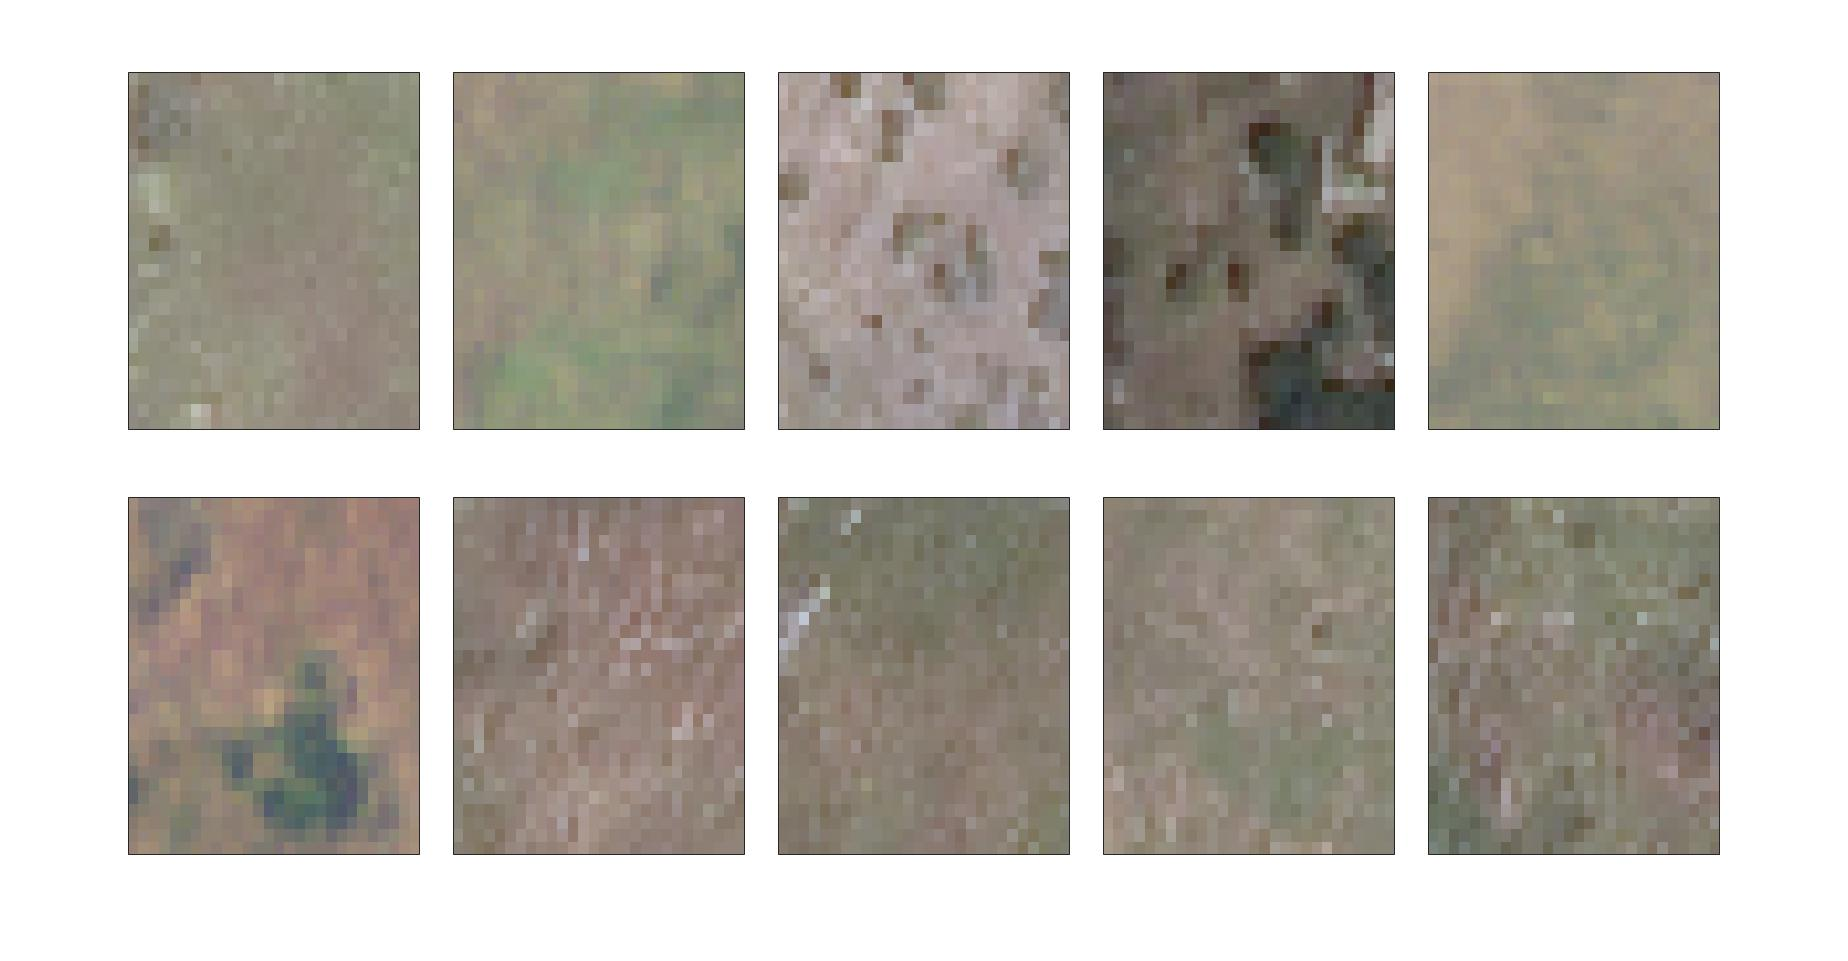
\includegraphics[width=2in]{BL_as_GL.jpg}}%
% \qquad
% \subfloat[][]{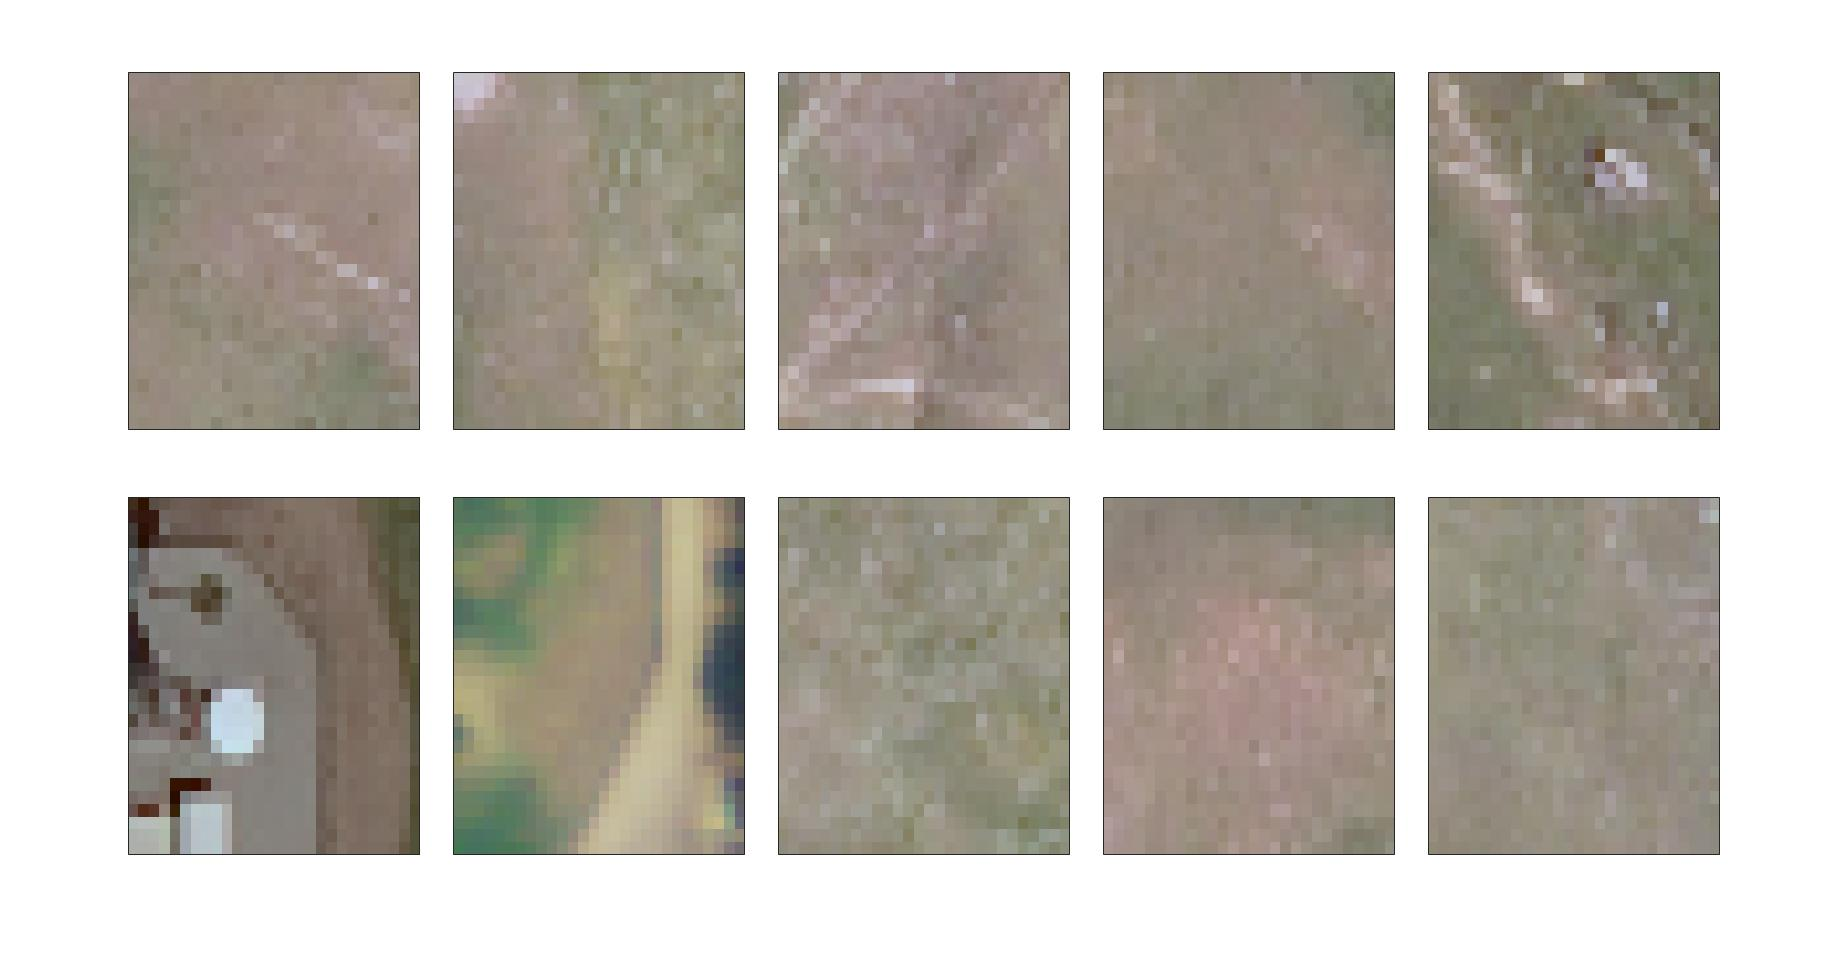
\includegraphics[width=2in]{GL_as_BL.jpg}}
% \caption{Example images with ground truth labels of (a) \emph{barrenland} and (b) \emph{grassland} which are mis-classified as each other.}%
% \label{fig: BL_GL}%
% \end{figure*}

\begin{figure*}[!t]%
\centering
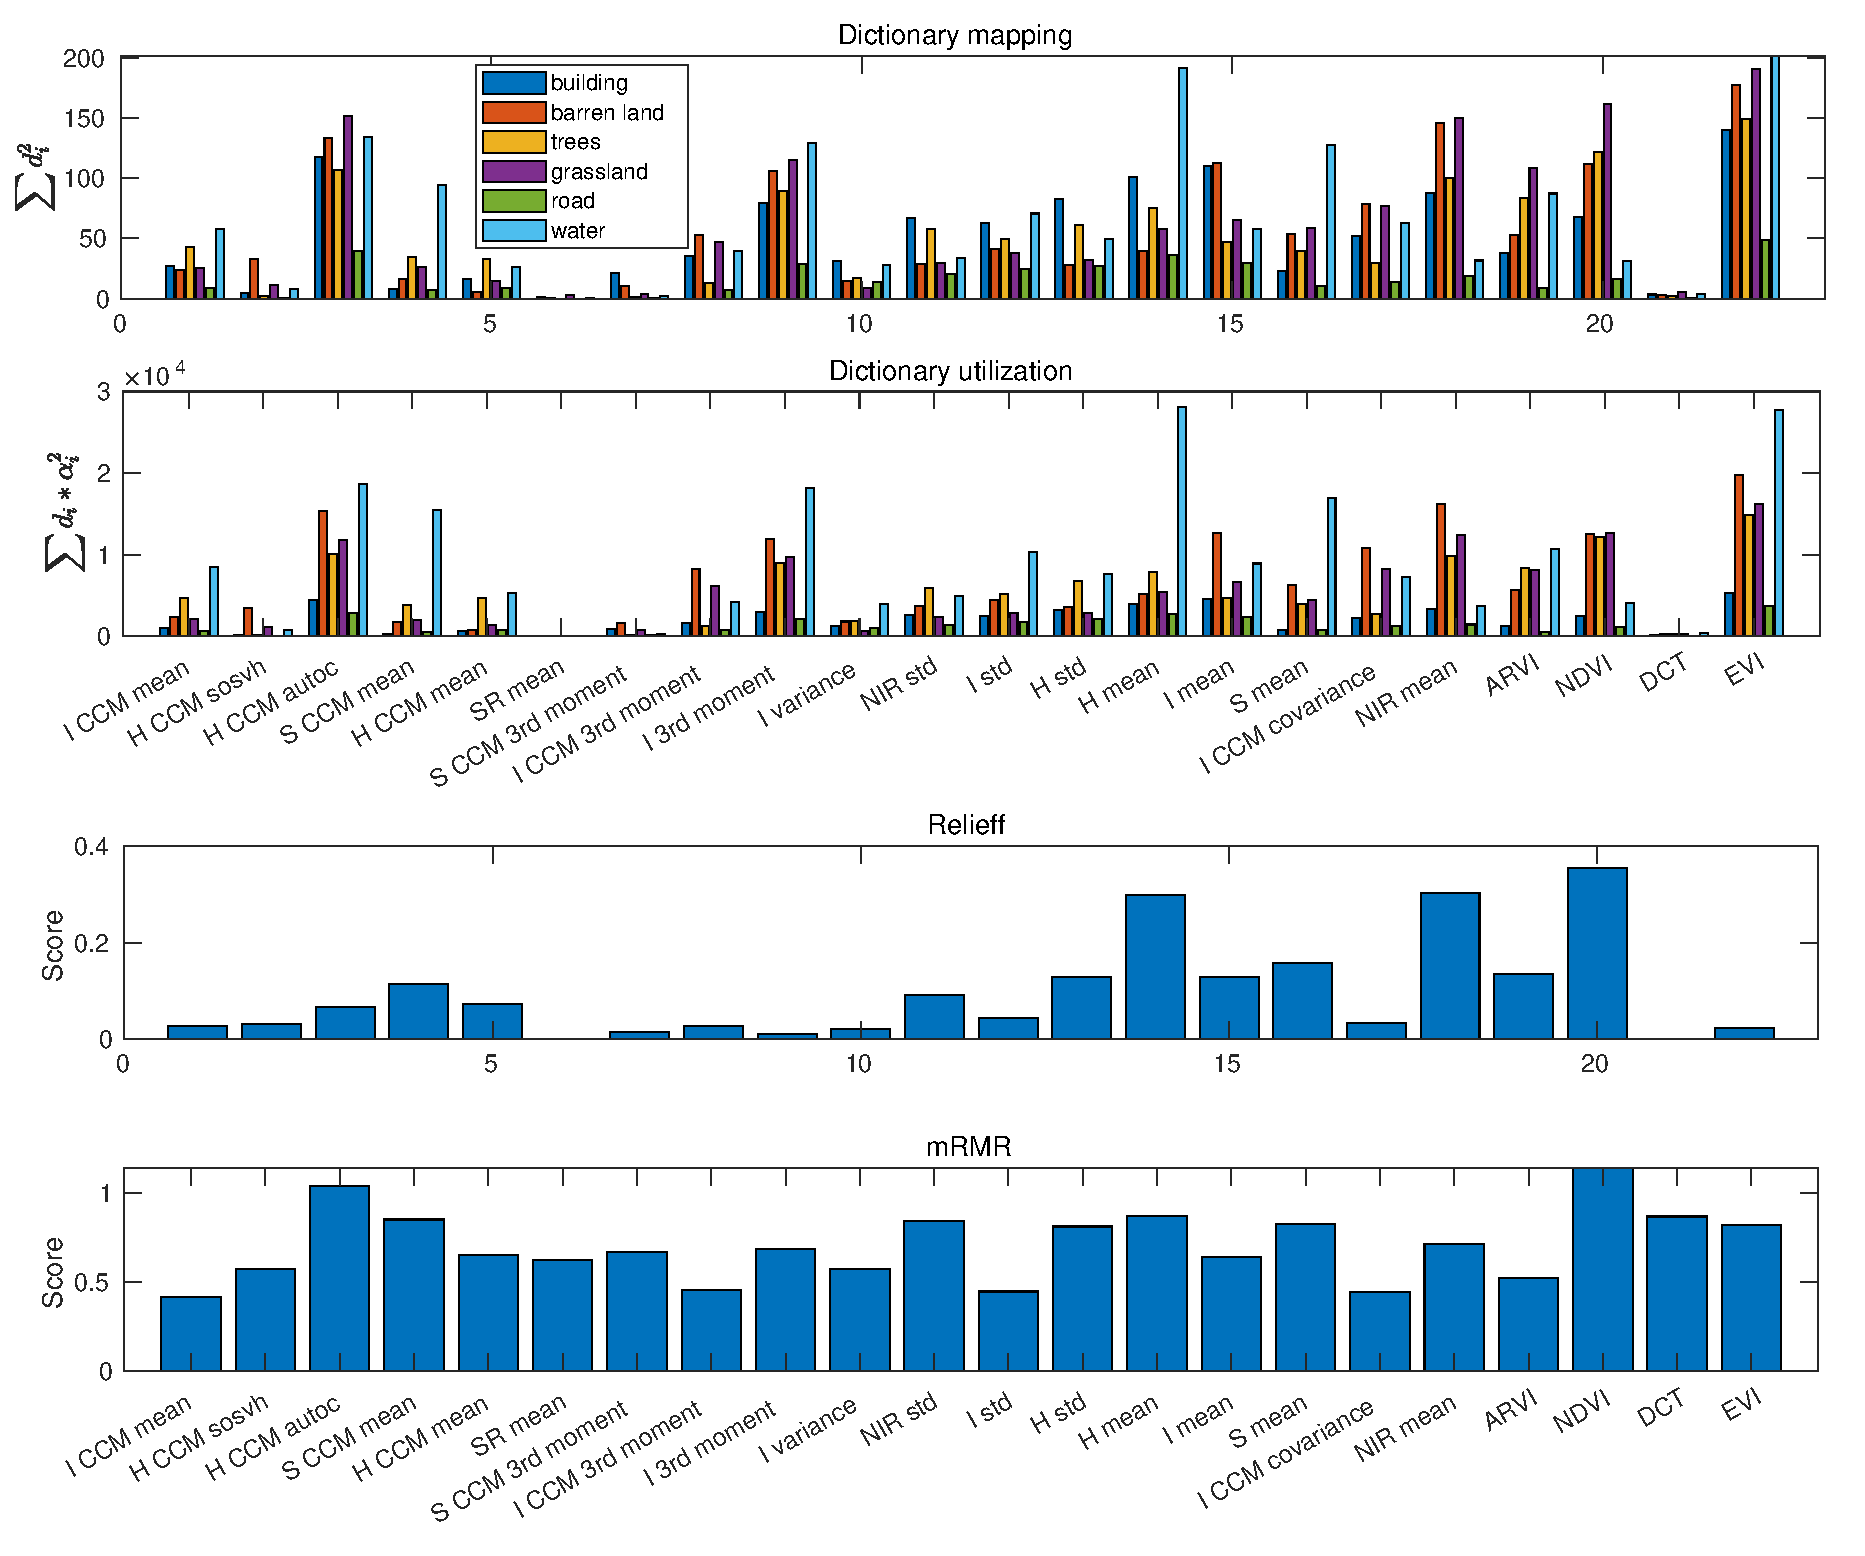
\includegraphics[width=\columnwidth]{figures/SR/Dict_FR.eps}
\caption{FR scores obtained using various methods on the Sat-6 dataset. The dictionary scores were obtained using frozen KSVD sparse representation.}%
\label{fig:FR}%
\end{figure*}


% \begin{figure*}[!t]
% \centering
% \subfloat[][]{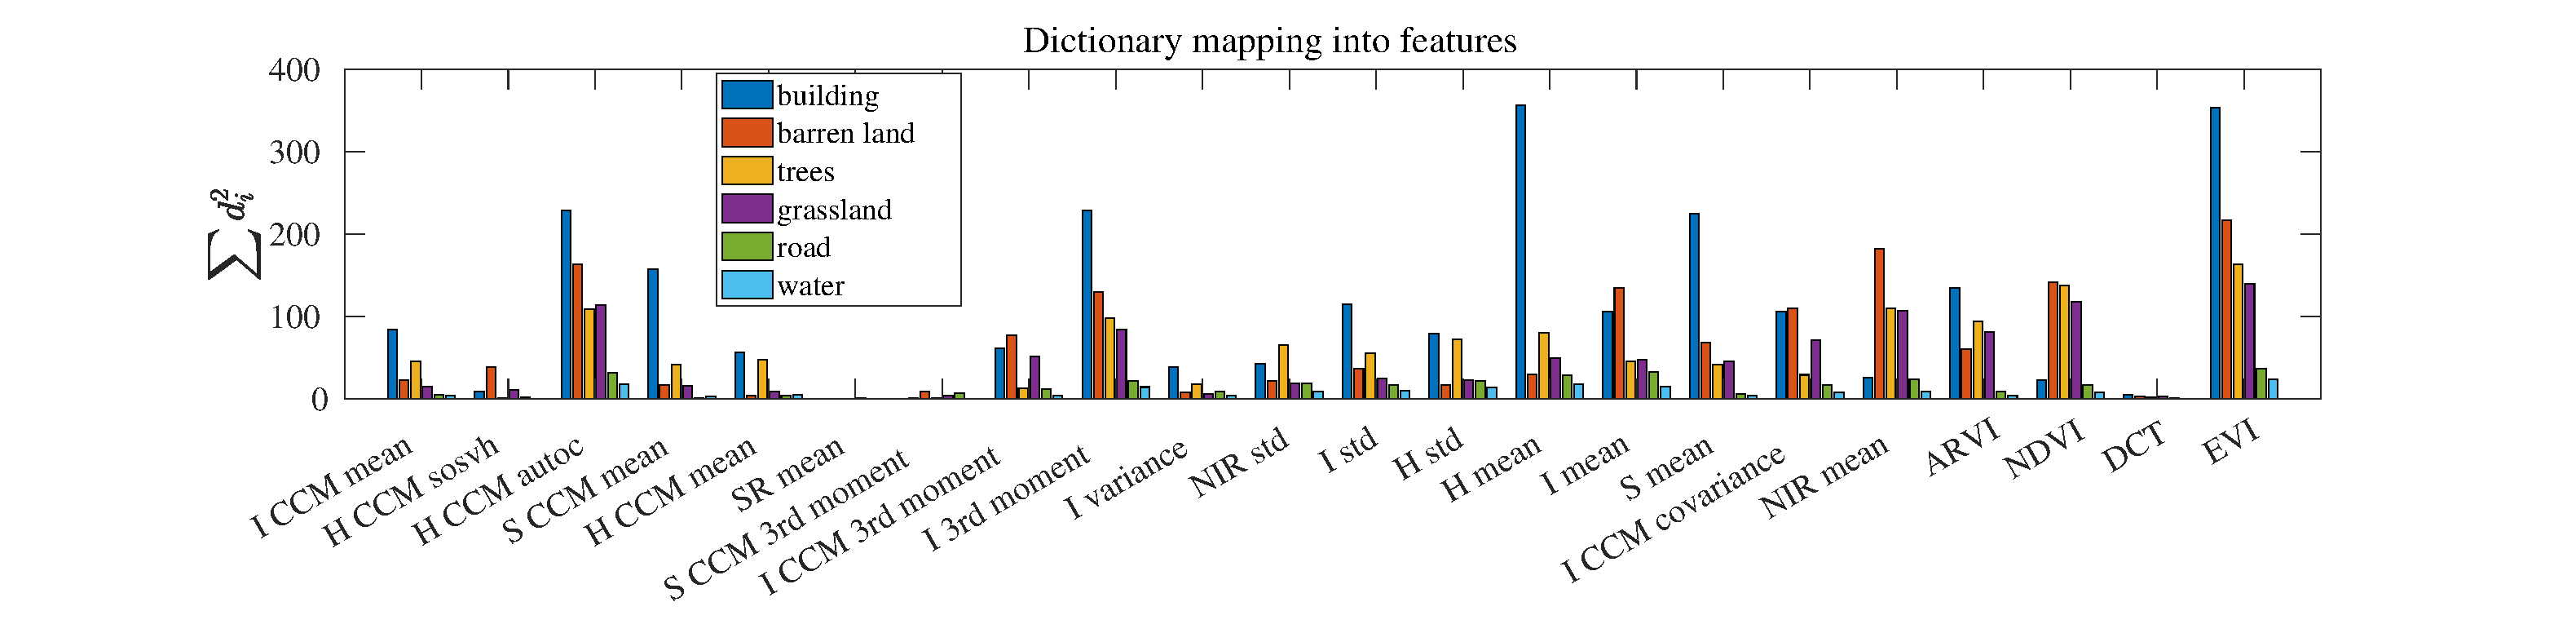
\includegraphics[width=7.2in]{Dict_map.eps}}\label{fig:dict_map}\\ 
% \subfloat[][]{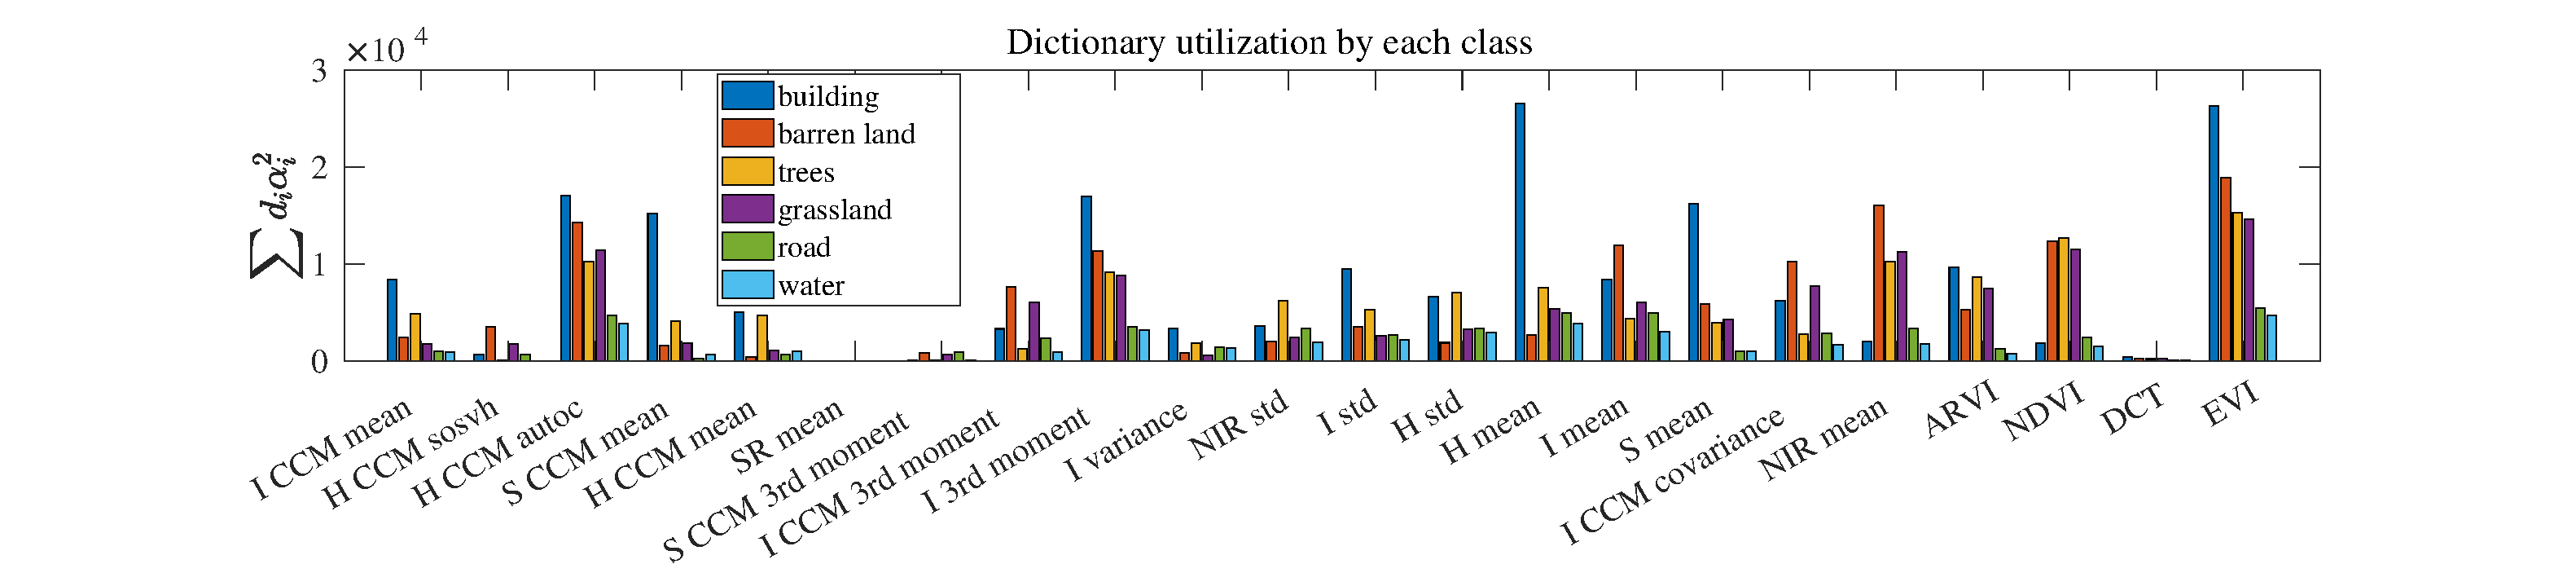
\includegraphics[width=7.2in]{Dict_util.eps}}\label{fig:dict_util}\\ 
% \subfloat[][]{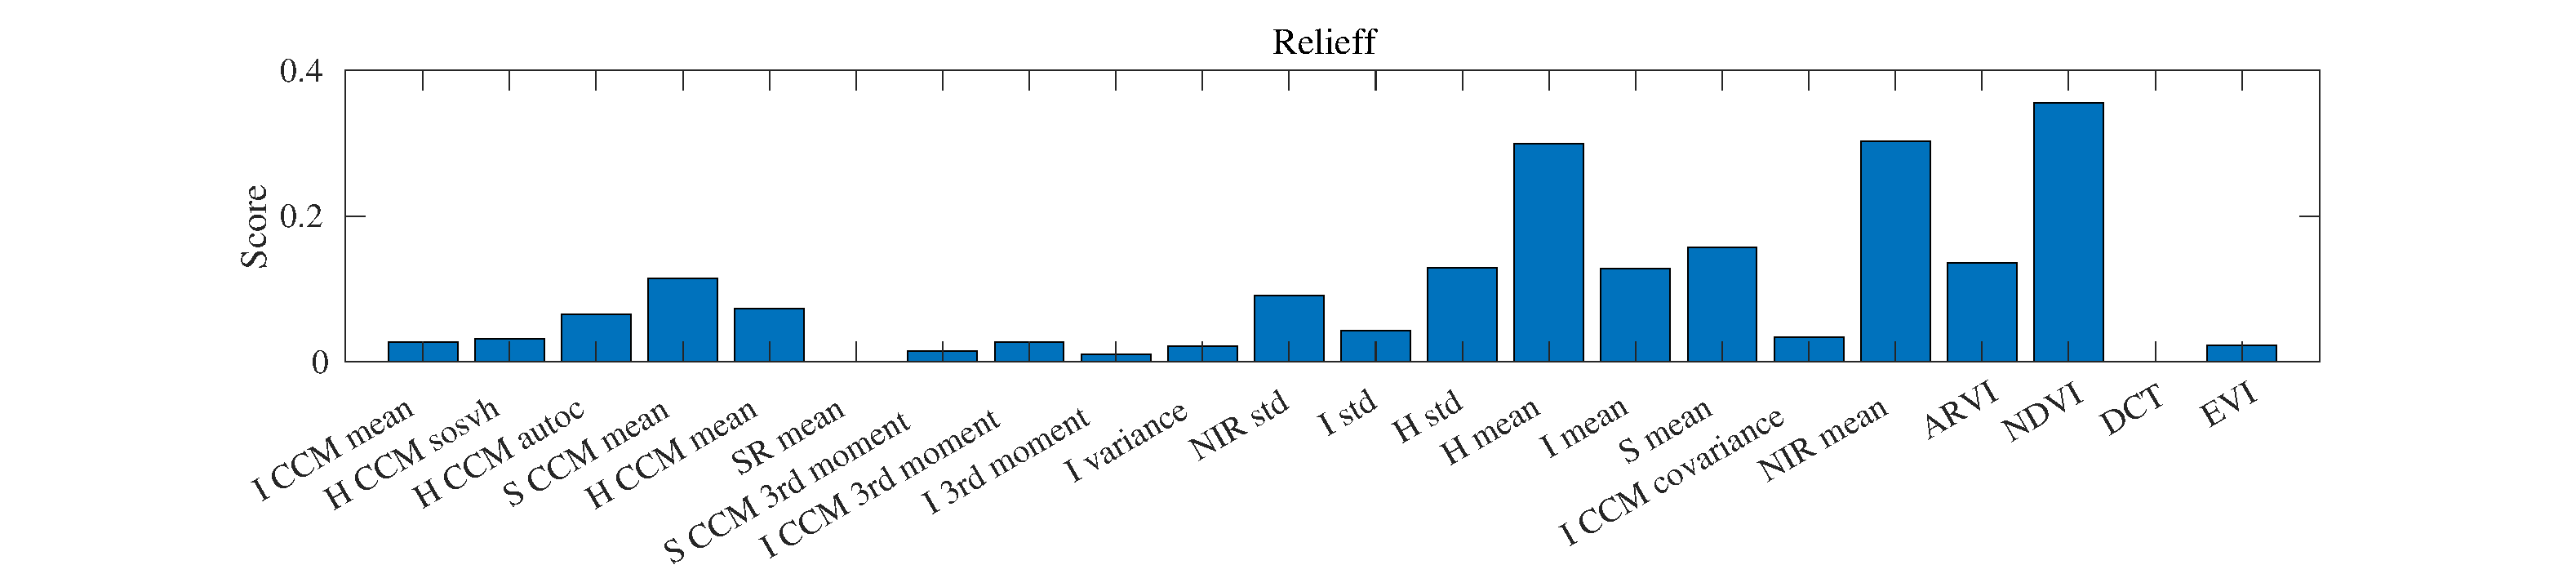
\includegraphics[width=7.2in]{Sat6_Releiff.eps}} \label{relieff}\\
% \subfloat[][]{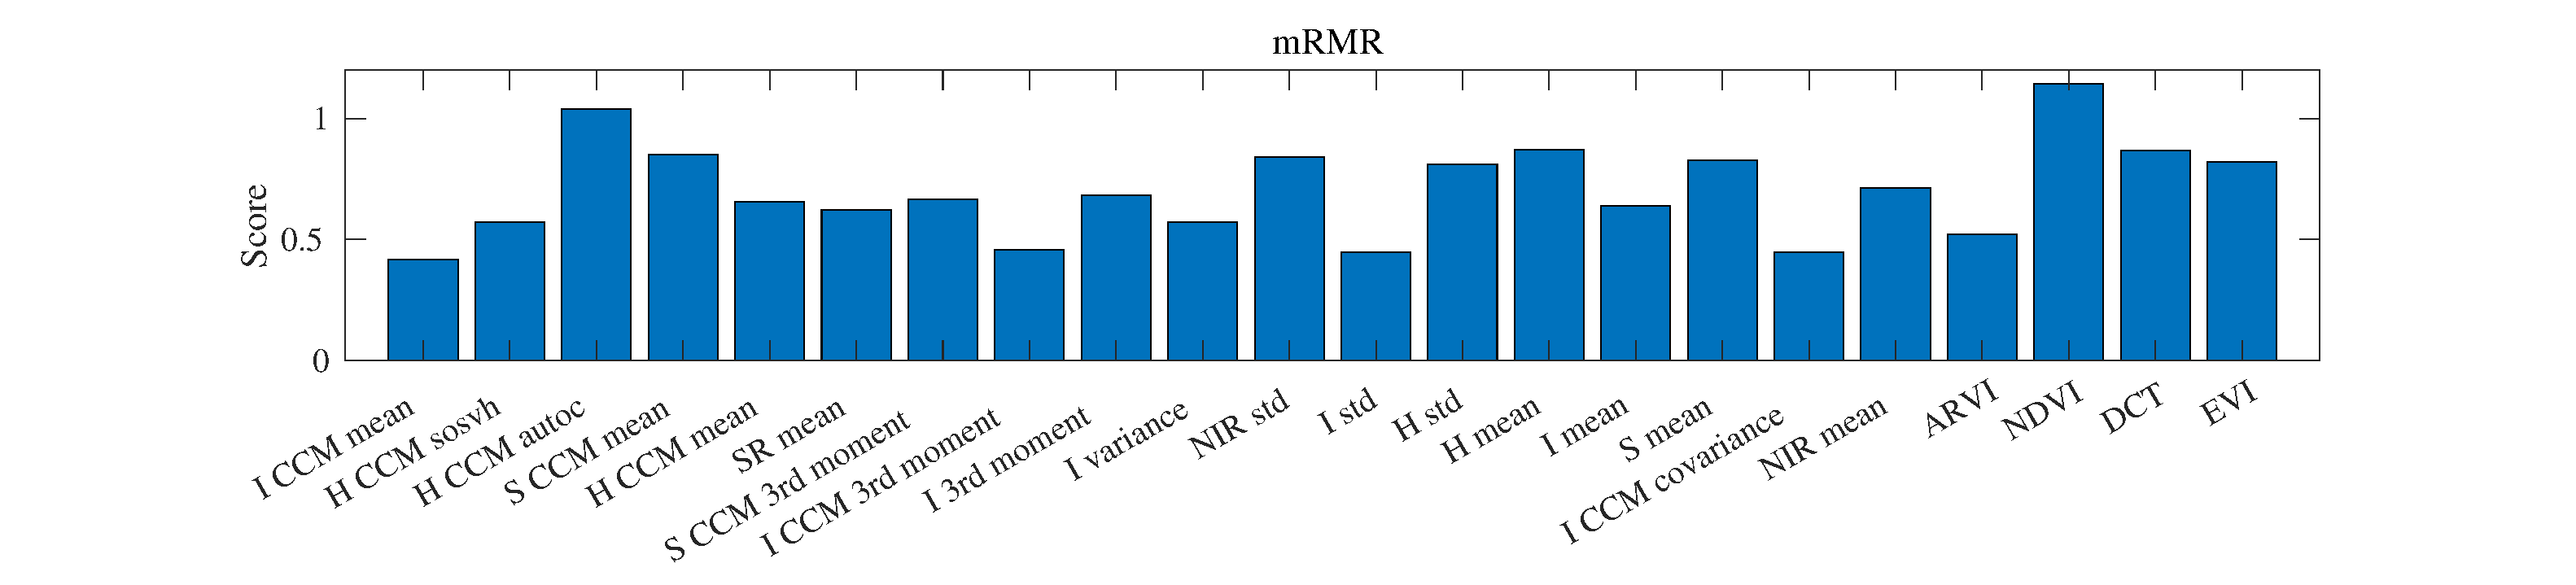
\includegraphics[width=7.2in]{Sat6_mRMR.eps}}\label{fig:mrmr}%
% \caption{Feature utilization by dictionary elements by class}%
% \label{fig:FR}%
% \end{figure*}

When we examine the dictionary atoms used by correctly and incorrectly classified images it can be observed that incorrectly classified images share some of the dictionary atoms that are mostly allocated to the other class. When we transform these dictionary elements back to the feature space we can identify the features that give similar parameters to the two classes, indicating that these features are not able to distinguish between the two classes. Hence, we can decide whether to replace the features or add new features that are capable of separating the two classes. Since our feature domain is considerably small this will not drastically increase the computational burden of the system for this example. This ability to identify the features responsible for misclassifications is not intuitively simple with deep networks and other FR methods. 

As an example, we can take a closer look at the most prevailing confusion between classes \emph{barren land} and \emph{grassland} in the Sat-6 dataset from the Frozen dictionary model. Most of the the misclassified images belonging to these classes contain soil and grass patches. For brevity, we do not present images of the misclassified data points, but the difficulty in producing accurate ground-truth labels likely contributes to the confusion and lower accuracy. This can be observed also in the misclassified \emph{building} class, where many of the images misclassified as \emph{roads} were parking lots. This, combined with the fact that \emph{roads} have very small training data, would accumulate to the low performance of the \emph{road} class. While a similar analysis could be done for images classified with a deep network, the linearity employed by dictionary learning and classification in this work allows for a more comprehensive analysis. 

Fig.\ref{fig:FR} shows the \emph{dictionary mapping} and the \emph{dictionary utilization} of the sparse coefficients used by dictionary elements projected into the original feature space from the frozen KSVD method on Sat-6 data. Since each dictionary atom is associated with a class, the class-wise metric analysis is performed on the original features. It also shows the FR done by the non-class specific Releiff and mRMR methods. Both proposed metrics perform in a similar fashion. While their scores are closer to the Relieff method they are also able to capture some important features predicted by mRMR method (e.g. \emph{H CCM autoc} and \emph{EVI}). The proposed methods also match the Relieff method in identifying SR mean and DCT as underutilized features.

The shortcomings of SR are well recorded in cases where an abundance of bare soil is present, and indices like Soil Adjusted Vegetation Indexes (SAVI) can be used to mitigate this problem\cite{Huete1988}. Due to the presence of similar texture in both \emph{barren land} and \emph{grassland} classes, its DCT components also give similar results. Since we have used a modified and more statistical version of the 22 features selected by\cite{Basu2015}, some features do not perform well with the sparse model. Using sparse coding and linear classifiers, we can identify, evaluate, and improve the necessary input features that might increase the performance of the classification.

Concerning classification performance between the two SR methods used, Frozen KSVD performs slightly better than the LC-KSVD in the Sat-6 dataset. This is possibly due to the strategy Frozen KSVD employs in taking class sizes into account and learning dictionary elements hierarchically. This enables the algorithm to produce dictionary atoms that specifically model the smaller classes. For the Sat-4 dataset, Frozen KSVD performs notably better than LC-KSVD\@. This may be due to the high variability of the \emph{none} class.

\section{Task 3: Hyperbolic graph embedding}